%%%%%%%%%%%%%%%%%%%%%%%%%%%%%%%%%%%%%%%%%
% Programming/Coding Assignment
% LaTeX Template
%
% This template has been downloaded from:
% http://www.latextemplates.com
%
% Original author:
% Ted Pavlic (http://www.tedpavlic.com)
%
% Note:
% The \lipsum[#] commands throughout this template generate dummy text
% to fill the template out. These commands should all be removed when 
% writing assignment content.
%
% This template uses a Perl script as an example snippet of code, most other
% languages are also usable. Configure them in the "CODE INCLUSION 
% CONFIGURATION" section.
%
%%%%%%%%%%%%%%%%%%%%%%%%%%%%%%%%%%%%%%%%%

%----------------------------------------------------------------------------------------
%	PACKAGES AND OTHER DOCUMENT CONFIGURATIONS
%----------------------------------------------------------------------------------------

\documentclass{article}

\usepackage{graphicx}
\usepackage{subfig}
\usepackage{amssymb}
\usepackage{multirow}
\usepackage{fancyhdr} % Required for custom headers
\usepackage{lastpage} % Required to determine the last page for the footer
\usepackage{extramarks} % Required for headers and footers
\usepackage[usenames,dvipsnames]{color} % Required for custom colors
\usepackage{graphicx} % Required to insert images
\usepackage{listings} % Required for insertion of code
\usepackage{courier} % Required for the courier font
\usepackage{lipsum} % Used for inserting dummy 'Lorem ipsum' text into the template
\usepackage{color} %red, green, blue, yellow, cyan, magenta, black, white
\usepackage[fleqn]{amsmath}
\usepackage{amsthm}
\usepackage{hyperref}
\DeclareMathOperator*{\argmax}{arg\,max}
\DeclareMathOperator*{\argmin}{arg\,min}
\definecolor{mygreen}{RGB}{28,172,0} % color values Red, Green, Blue
\definecolor{mylilas}{RGB}{170,55,241}
% Margins
\topmargin=-0.45in
\evensidemargin=0in
\oddsidemargin=0in
\textwidth=6.5in
\textheight=9.0in
\headsep=0.25in

\linespread{1.1} % Line spacing

% Set up the header and footer
\pagestyle{fancy}
\lhead{\hmwkAuthorName} % Top left header
\chead{\hmwkClass\ (\hmwkClassInstructor\ \hmwkClassTime): \hmwkTitle} % Top center head
\rhead{\firstxmark} % Top right header
\lfoot{\lastxmark} % Bottom left footer
\cfoot{} % Bottom center footer
\rfoot{Page\ \thepage\ of\ \protect\pageref{LastPage}} % Bottom right footer
\renewcommand\headrulewidth{0.4pt} % Size of the header rule
\renewcommand\footrulewidth{0.4pt} % Size of the footer rule

\setlength\parindent{0pt} % Removes all indentation from paragraphs

%----------------------------------------------------------------------------------------
%	CODE INCLUSION CONFIGURATION
%----------------------------------------------------------------------------------------

\definecolor{MyDarkGreen}{rgb}{0.0,0.4,0.0} % This is the color used for comments
\lstloadlanguages{Perl} % Load Perl syntax for listings, for a list of other languages supported see: ftp://ftp.tex.ac.uk/tex-archive/macros/latex/contrib/listings/listings.pdf
\lstset{language=Perl, % Use Perl in this example
        frame=single, % Single frame around code
        basicstyle=\small\ttfamily, % Use small true type font
        keywordstyle=[1]\color{Blue}\bf, % Perl functions bold and blue
        keywordstyle=[2]\color{Purple}, % Perl function arguments purple
        keywordstyle=[3]\color{Blue}\underbar, % Custom functions underlined and blue
        identifierstyle=, % Nothing special about identifiers                                         
        commentstyle=\usefont{T1}{pcr}{m}{sl}\color{MyDarkGreen}\small, % Comments small dark green courier font
        stringstyle=\color{Purple}, % Strings are purple
        showstringspaces=false, % Don't put marks in string spaces
        tabsize=5, % 5 spaces per tab
        %
        % Put standard Perl functions not included in the default language here
        morekeywords={rand},
        %
        % Put Perl function parameters here
        morekeywords=[2]{on, off, interp},
        %
        % Put user defined functions here
        morekeywords=[3]{test},
       	%
        morecomment=[l][\color{Blue}]{...}, % Line continuation (...) like blue comment
        numbers=left, % Line numbers on left
        firstnumber=1, % Line numbers start with line 1
        numberstyle=\tiny\color{Blue}, % Line numbers are blue and small
        stepnumber=5 % Line numbers go in steps of 5
}

\lstset{language=Matlab,%
    %basicstyle=\color{red},
    breaklines=true,%
    morekeywords={matlab2tikz},
    keywordstyle=\color{blue},%
    morekeywords=[2]{1}, keywordstyle=[2]{\color{black}},
    identifierstyle=\color{black},%
    stringstyle=\color{mylilas},
    commentstyle=\color{mygreen},%
    showstringspaces=false,%without this there will be a symbol in the places where there is a space
    numbers=left,%
    numberstyle={\tiny \color{black}},% size of the numbers
    numbersep=9pt, % this defines how far the numbers are from the text
    emph=[1]{for,end,break},emphstyle=[1]\color{red}, %some words to emphasise
    %emph=[2]{word1,word2}, emphstyle=[2]{style},    
}

% Creates a new command to include a perl script, the first parameter is the filename of the script (without .pl), the second parameter is the caption
\newcommand{\perlscript}[2]{
\begin{itemize}
\item[]\lstinputlisting[caption=#2,label=#1]{#1.pl}
\end{itemize}
}


%----------------------------------------------------------------------------------------
%	DOCUMENT STRUCTURE COMMANDS
%	Skip this unless you know what you're doing
%----------------------------------------------------------------------------------------

% Header and footer for when a page split occurs within a problem environment
\newcommand{\enterProblemHeader}[1]{
\nobreak\extramarks{#1}{#1 continued on next page\ldots}\nobreak
\nobreak\extramarks{#1 (continued)}{#1 continued on next page\ldots}\nobreak
}

% Header and footer for when a page split occurs between problem environments
\newcommand{\exitProblemHeader}[1]{
\nobreak\extramarks{#1 (continued)}{#1 continued on next page\ldots}\nobreak
\nobreak\extramarks{#1}{}\nobreak
}

\setcounter{secnumdepth}{0} % Removes default section numbers
\newcounter{homeworkProblemCounter} % Creates a counter to keep track of the number of problems

\newcommand{\homeworkProblemName}{}
\newenvironment{homeworkProblem}[1][Problem \arabic{homeworkProblemCounter}]{ % Makes a new environment called homeworkProblem which takes 1 argument (custom name) but the default is "Problem #"
\stepcounter{homeworkProblemCounter} % Increase counter for number of problems
\renewcommand{\homeworkProblemName}{#1} % Assign \homeworkProblemName the name of the problem
\section{\homeworkProblemName} % Make a section in the document with the custom problem count
\enterProblemHeader{\homeworkProblemName} % Header and footer within the environment
}{
\exitProblemHeader{\homeworkProblemName} % Header and footer after the environment
}

\newcommand{\problemAnswer}[1]{ % Defines the problem answer command with the content as the only argument
\noindent\framebox[\columnwidth][c]{\begin{minipage}{0.98\columnwidth}#1\end{minipage}} % Makes the box around the problem answer and puts the content inside
}

\newcommand{\homeworkSectionName}{}
\newenvironment{homeworkSection}[1]{ % New environment for sections within homework problems, takes 1 argument - the name of the section
\renewcommand{\homeworkSectionName}{#1} % Assign \homeworkSectionName to the name of the section from the environment argument
\subsection{\homeworkSectionName} % Make a subsection with the custom name of the subsection
\enterProblemHeader{\homeworkProblemName\ [\homeworkSectionName]} % Header and footer within the environment
}{
\enterProblemHeader{\homeworkProblemName} % Header and footer after the environment
}

%----------------------------------------------------------------------------------------
%	NAME AND CLASS SECTION
%----------------------------------------------------------------------------------------

\newcommand{\hmwkTitle}{Assignment2} % Assignment title
\newcommand{\hmwkDueDate}{\today} % Due date
\newcommand{\hmwkClass}{CS299:Machine Learning} % Course/class
\newcommand{\hmwkClassTime}{} % Class/lecture time
\newcommand{\hmwkClassInstructor}{Andrew Ng} % Teacher/lecturer
\newcommand{\hmwkAuthorName}{Bryan Zhang} % Your name


%----------------------------------------------------------------------------------------
% PROBABILITY SHORT CUT
%----------------------------------------------------------------------------------------
\newcommand{\p}[1]{p(#1)}
\newcommand{\abs}[1]{|#1|}
\newcommand{\1}[1]{1\{#1\}}
\newcommand{\equations}[1]{
	\begin{equation}
	     \begin{split}
	     #1
	     \end{split}
	\end{equation}
}
\newcommand{\upi}[1]{#1^{(i)}}
\newtheorem{theorem}{Theorem}
%----------------------------------------------------------------------------------------
%	TITLE PAGE
%----------------------------------------------------------------------------------------

\title{
\vspace{2in}
\textmd{\textbf{\hmwkClass:\ \hmwkTitle}}\\
\normalsize\vspace{0.1in}\small{Due\ on\ \hmwkDueDate}\\
\vspace{0.1in}\large{\textit{\hmwkClassInstructor\ \hmwkClassTime}}
\vspace{3in}
}

\author{\textbf{\hmwkAuthorName}}
\date{} % Insert date here if you want it to appear below your name

%----------------------------------------------------------------------------------------

\begin{document}

\maketitle

%----------------------------------------------------------------------------------------
%	TABLE OF CONTENTS
%----------------------------------------------------------------------------------------

%\setcounter{tocdepth}{1} % Uncomment this line if you don't want subsections listed in the ToC

\newpage
\tableofcontents


%----------------------------------------------------------------------------------------
%	PROBLEM 1: Logistic Regression: Training stability
%----------------------------------------------------------------------------------------

% To have just one problem per page, simply put a \clearpage after each problem

\begin{homeworkProblem}
 I answer the subquestions in a more convenient order.
 \subsection{1(a)}{
 The Most noticeable difference is that logistic regression converges quickly on dataset A but seems never converges for dataset B. \par
 For dataset A, it only took 30395 iteration to fulfill the 1e-15 error margin. But for dataset B, the algorithm are still running even for 16490000 iterations.
}

\subsection{1(d)}{
    First of all, Let's formulate the gradient ascent update rules used by logistic regression algorithm  in the $lr_debug.py$.
    \begin{equation}
        \theta_j = \theta_j +  \alpha(\frac{1}{m}\sum_{i = 1}^{m} x^{(i)}y^{(i)}\frac{1}{1 + e^{y^{(i)}x^{(i)}\cdot \theta^T}})
    \end{equation}
    Then we have to know what this update rule is maximizing. My guess is the log likelihood of being predicted correctly. After we compute the gradient, this can be proved.
    Assuming that the m training examples were generated independently. we can then write down the likelihood of the parameter as
    \begin{equation}
    \begin{split}
             L(\theta) &= p(Y|X;\theta) \\
                       &= \prod_{i = 1}^{m}(1 - p^{(i)}) \\
             p^{(i)}   &=  \frac{1}{1 + e^{y^{(i)}x^{(i)}\cdot \theta^T}} \\
             \gamma^{(i)} &= y^{(i)}x^{(i)}\cdot \theta^T
    \end{split}
    \end{equation}
    You can see intuitively that $\gamma^{(i)}$ will be negative if the algorithm makes a mistake, which will make $p^{(i)}$ bigger thus $L(\theta)$ smaller. As before, it will be easier to maximize the log likelihood:
    \begin{equation}
    \begin{split}
             l(\theta) &= log(\sqrt[m]{L(\theta)}) \\ 
                       &= \frac{1}{m}\sum_{i = 1}^{m}log(1 - p^{(i)}) \\
    \end{split}
    \end{equation}
    Now, to maximize our log likelihood, we use the gradient ascent:
    \begin{equation}
    \begin{split}
             \nabla_\theta l(\theta) &= \frac{1}{m}\sum_{i = 1}^{m}\nabla_\theta log(1 - p^{(i)}) \\     
                                     &= \frac{1}{m}\sum_{i = 1}^{m} -\frac{1}{1 - p^{(i)}} \nabla_\theta p^{(i)}  \\
                                     &= \frac{1}{m}\sum_{i = 1}^{m} -\frac{ 1 + e^{y^{(i)}x^{(i)}\cdot \theta^T}}{e^{y^{(i)}x^{(i)}\cdot \theta^T}}
                                        (- \frac{1}{(1 + e^{y^{(i)}x^{(i)}\cdot \theta^T})^2})e^{y^{(i)}x^{(i)}\cdot \theta^T}y^{(i)}x^{(i)} \\
                                     &= \frac{1}{m}\sum_{i = 1}^{m} \frac{1}{1 + e^{y^{(i)}x^{(i)}\cdot \theta^T}} y^{(i)}x^{(i)} \\
                                     &= \frac{1}{m}\sum_{i = 1}^{m} p^{(i)} y^{(i)}x^{(i)}
    \end{split}
    \end{equation}
    q.e.d. The logistic regression is try to maximizing the probability of the margins being positive. Geometrically, minimizing the logistic regression loss means the maximizing the margins toward a positive direction. 
    As for Support Vector Machine, I believe it will help. Since this time, the svm is trying to maximize the biggest margins rather than the sum of all margins, which makes it more robust for discontinuity. 
    }
    \subsection{1(b)} {
        \textbf{My hypothesis: data set B can have $\theta$s with difference more than $3e^{-15}$ but which make the maximum margins.} in other words, there is a flat discontinuity for dataset B, while the big gradient is just overshoot theta on the edges of the flat discontinuity, which is bigger than the required convergence condition. For dataset A, this is  not the case. Since for dataset A, mistakes has already been made. The separating line is just making the margins bigger. Also along separating line, dataset A has more data points to confine the line than dataset B. You can see the visualization for the dataset A's training process at \href{https://www.youtube.com/watch?v=y-r4V6zWyIk}{here} and for dataset B at \href{https://www.youtube.com/watch?v=6NFWGIuumPE}{here}.

        \begin{center}
           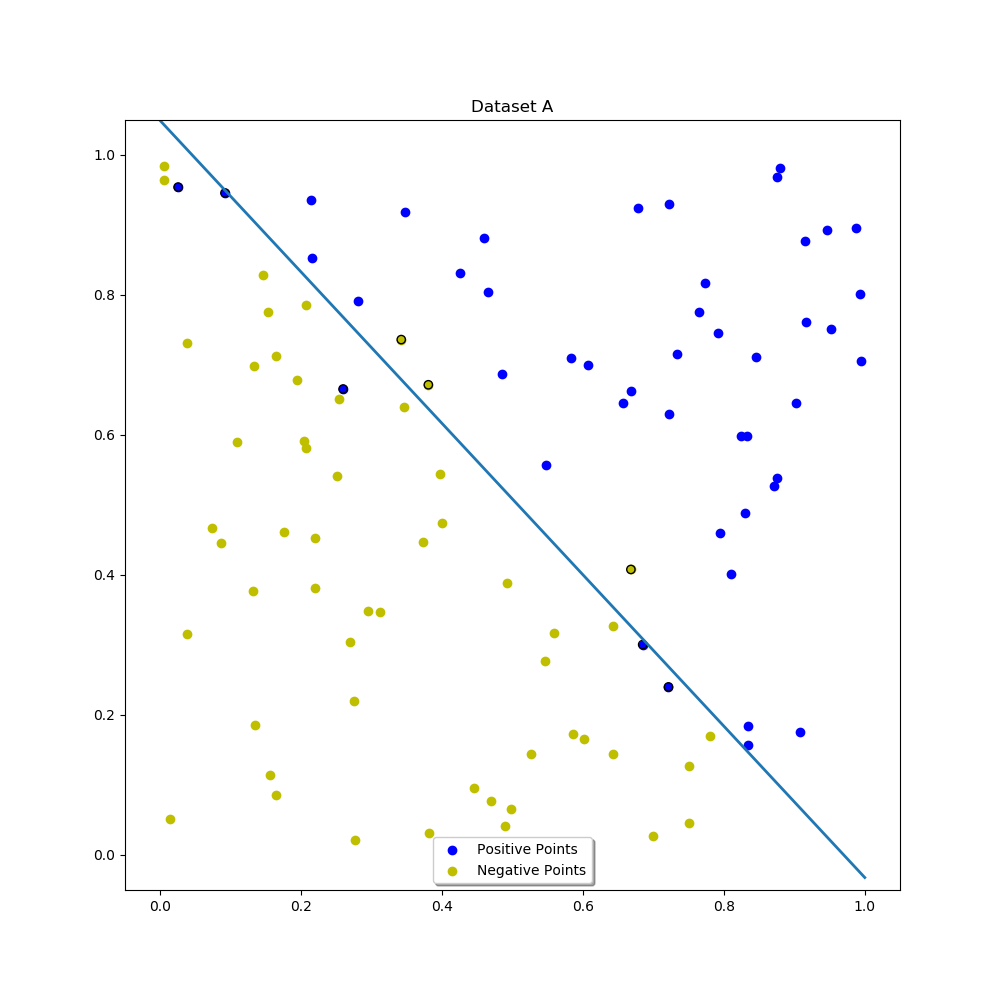
\includegraphics[width=0.8\textwidth]{lr_a.png}
           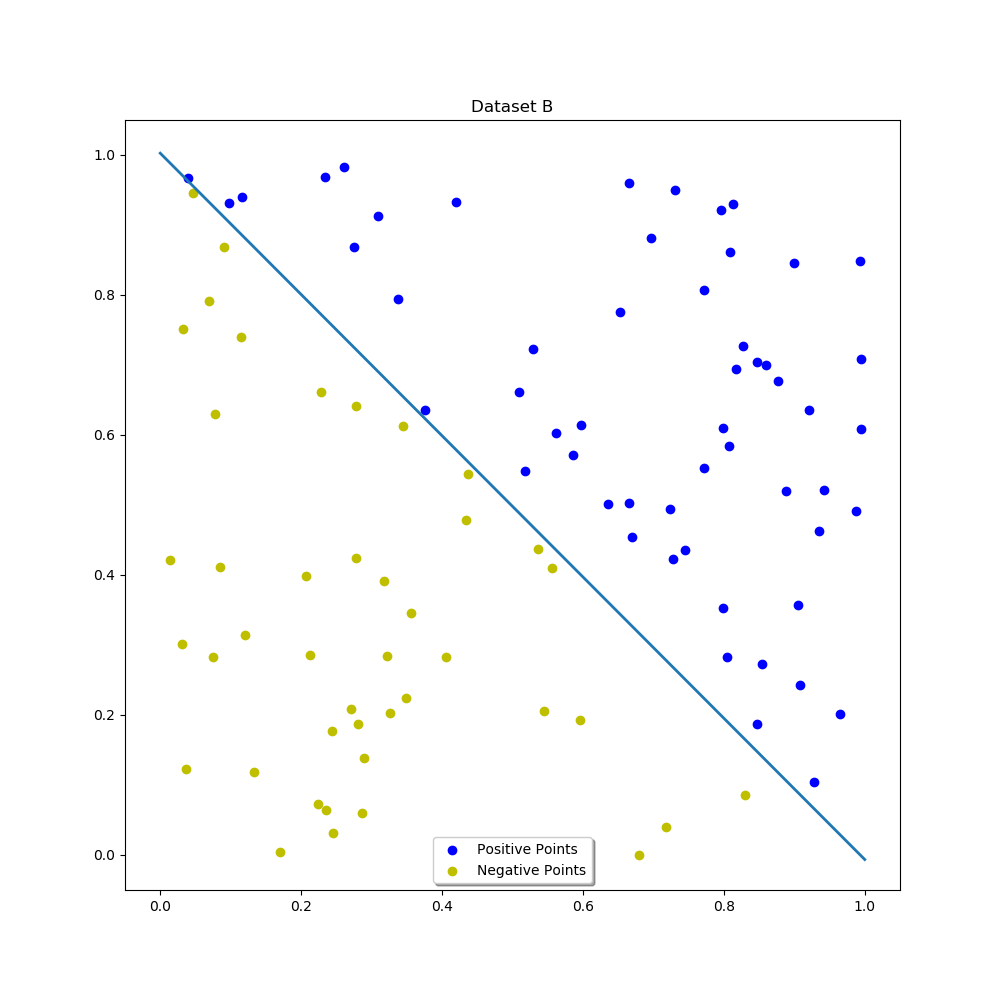
\includegraphics[width=0.8\textwidth]{lr_b.png}
        \end{center}
        
        }

    \subsection{1(c)} {
     \subsubsection{i.Using a different constant learning rate} {
         This won't help. Because if we slow the learning rate then to achieve the none-mistake separating line, the algorithms will take more iterations than the current learning rate. If we  accelerate the learning rate, after achieving the none-mistakes separating line, the algorithm will not be stable since the current learning rate has already overshoot the line between edges of the falt discontinuity. 
         The experiment results
         \begin{center}
          \begin{tabular}{ | l | c |}
            \hline
            learning rate & iterations \\ \hline
            1e-1 & $>86000$ \\ \hline
            1e-2 & $>$86000 \\ \hline
            1 &  $>$86000 \\ \hline
            100 & $>$86000 \\ \hline
            1000 & $>$86000(Overflow Warning) \\ \hline
          \end{tabular}
        \end{center}
     }
     \subsubsection{ii.Decreasing the learning rate over time}{
       This will help. Because it will eliminate the iterations that overshoots and don't contribute the final accuracy. However, I found the decreasing factor matters two. With higher decreasing order, the training converges before it reaches the good separating line. While if the factor has too slow order, then the training takes too many iterations. Below is my experiment result:
        \begin{center}
          \begin{tabular}{| c | c | c | c |}
            \hline
            decreasing factor & learning rate & iterations & number of mistakes \\ \hline
            \multirow{2}{4em}{$\frac{1}{t^2}$} & 10 & 12 & 43\\  
            & 100 & 12 & 9 \\ \hline
            \multirow{2}{4em}{$\frac{1}{t}$} & 10 & 18 & 14\\ 
            & 100 & 19 & 7 \\ \hline
            \multirow{2}{4em}{$\frac{1}{\sqrt[]{t}}$} & 10 & 29 & 21\\  
            & 100 & 29 & 7 \\ \hline
            \multirow{2}{4em}{$\frac{1}{log(t)}$} & 10 & $>$86000(divide by zero warning) & Unkown\\ 
            & 100 & $>$86000(divide by zero warning) & Unkown\\ \hline
          \end{tabular}
        \end{center}
        Below is the  best performance under the learning rate = 100 and decreasing factor =  $\frac{1}{\sqrt[]{t}}$.
        \begin{center}
             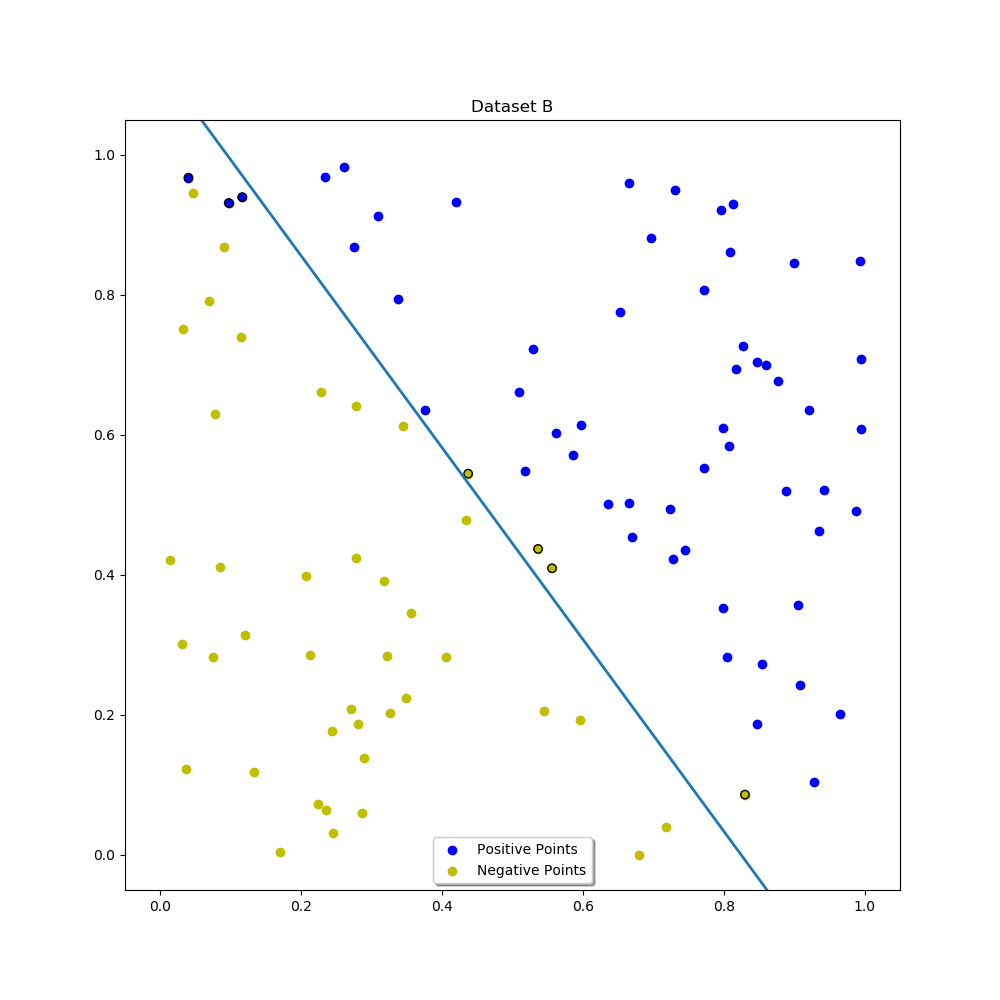
\includegraphics[width=0.8\textwidth]{lr_b_decrease_learning_rate.png}
        \end{center}
     }
     \subsubsection{iii. Add a regularization term to the loss function.} {
        I will add a term $||\theta||^2$ to the loss and thus a term of $2\theta$   to the gradient. This doesn't help.Because the regularization is to penalize big thetas and give reward to more sparse thetas, which can't stabilize the overshoot in training dataset B.
     }
     \subsubsection{iv. linearly scale of input features} {
     This won't help. Because linear scaling of the input features will have no effect of the line slop and intercept, both of which loose the scale when they are computed by dividing of c.
     Here is my experiment result:
         \begin{center}
          \begin{tabular}{ | l | c |}
            \hline
            scaling factor & iterations \\ \hline
            1 & $>86000$ \\ \hline
            0.5 & $>$86000 \\ \hline
            0.1 &  $>$86000 \\ \hline
            1e-2 & $>$86000 \\ \hline
            1e-4 & $>$86000 \\ \hline
          \end{tabular}
        \end{center}
     }
     \subsubsection{v. Add zero-mean Gaussian noise to the training data or labels} {
         This won't help either. Since once they are summed together to be theta the noise cancels out.
     }
    }
\end{homeworkProblem}
%----------------------------------------------------------------------------------------



%----------------------------------------------------------------------------------------
%   PROBLEM 2: Model Calibration 
%----------------------------------------------------------------------------------------

% To have just one problem per page, simply put a \clearpage after each problem

\begin{homeworkProblem}
  \subsection{a}{
  In logistic regression, we want to maximize the log likelihood:
  \begin{equation}
    \begin{split}
             l(\theta) &=  \sum_{i  = 1}^{m}y^{(i)}h(x^{(i)}) + (1 - y^{(i)})log(1-h(x^{(i)}))\\
    \end{split}
    \end{equation}
    This time, instead of updating by gradient, we simply put its gradient to zero. And we have confidence to say that in this way, the parameter is also the learned parameter.
      \begin{equation}
    \begin{split}
             \nabla_{\theta} l(\theta) &=  x^T\cdot(y - h_{\theta}(x))\ = 0\
    \end{split}
    \end{equation}
    If we  look at the bias term column in x, we can have
    \begin{equation}
    \begin{split}
              \sum_{i=1}^m (y^{(i)} - h_{\theta}(x^{(i)})) &= 0\\
    \end{split}
    \end{equation}
    Relocating sum of probabilities and sum of the labels to opposite sides of the equation, we can prove the property.
  }

  \subsection{b} {
  If the model achieves perfect accuracy, which means it will predict all positive example with 1 and negative with 0.Then  both sides of the property equation will be zero if the interval doesn't include 1. When it do includes 1, the proper equation still holds to be 1. Thus The model who achieves perfect accuracy is perfectly calibrated.
   But a perfect calibrated  binary classifier can not achieve perfect accuracy. Because we can easily find a counter-example. Let half of example be negative and the prediction probabilities for all examples are $\frac{1}{2}$. Thus for intervals that contains $\frac{1}{2}$, the property holds to be  one half on both sides of the equations. For intervals that don't contains $\frac{1}{2}$, the both sides of the equations are zero, which guarantees the property. Thus the model must be perfectly calibrated but can't achieve perfect accuracy.
  }
  \subsection{c} {
  the objective function now is 
   \begin{equation}
    \begin{split}
              J(\theta) &= \frac{1}{2} \sum_{i=1}^{m}(h_{\theta}(x^{(i)}) - y^{(i)})^2 + \frac{1}{2} \theta ^2\\
    \end{split}
    \end{equation}
    Now we compute its gradient to $\theta$.
    \begin{equation}
    \begin{split}
              \nabla_{\theta} J(\theta) &= x^T \cdot (h_{\theta}(x^{(i)}) - y^{(i)}) + \theta\\
    \end{split}
    \end{equation}
    Then we set the gradient to zero to find the $ \argmin_\theta J(\theta)B$.
    \begin{equation}
    \begin{split}
               x^T \cdot (h_{\theta}(x^{(i)}) - y^{(i)}) &=  - \theta\\
    \end{split}
    \end{equation}
    Still we investigate the intercept term.
    \begin{equation}
    \begin{split}
              \sum_{i=1}^m P(y^{(i) = 1}|x^{(i)};\theta) &= \sum_{i=1}^m \textbf{1}\{y^{(i)} = 1\}  - \theta_1\\
    \end{split}
    \end{equation}
    Thus, the $L_2$ regularization shift the probabilities toward zero by the extent of $\theta_1$. This means Bigger $\theta_1$ will predict lower probabilities.
  }
\end{homeworkProblem}

%----------------------------------------------------------------------------------------



%----------------------------------------------------------------------------------------
%   PROBLEM 3: Baysian Logistic Regression and weight decay 
%----------------------------------------------------------------------------------------
\begin{homeworkProblem}
    If we assume that 
    \equations{
    ||\theta_{MAP}||_2 > ||\theta_{ML}||_2
    } 
    Thus, $\theta_{MAP}$ is not equal to $\theta_{ML}$, the $\argmax_{\theta} \prod_{i=1}^mp(y^{(i)}|x^{(i)}, \theta)$, which gives $p(y^{(i)}|x^{(i)}, \theta_{MAP}) < p(y^{(i)}|x^{(i)}, \theta_{ML})$. Also  if prior $\theta \sim \mathcal{N}(0, \tau^2 I)$, $p(\theta_{MAP}) < P(\theta_{ML})$, for our assumption guarantees that $\theta_{MAP}$ are more away from the mean point zero. 
    Using above two inequality, we can have this inequality,
    \equations{
     p(\theta_{MAP})\prod_{i=1}^mp(y^{(i)}|x^{(i)}, \theta_{MAP}) < p(\theta_{ML})\prod_{i=1}^mp(y^{(i)}|x^{(i)}, \theta_{ML})
     } 
     This inequality contradicts our condition that,
     \equations{
      \theta_{MAP}| = \argmax_\theta{p(\theta)\prod_{i=1}^mp(y^{(i)}|x^{(i)}, \theta)}
     } q.e.d
\end{homeworkProblem}
    
%----------------------------------------------------------------------------------------

%----------------------------------------------------------------------------------------
%   PROBLEM 4: Constructing kernels 
%----------------------------------------------------------------------------------------
\begin{homeworkProblem}
\subsection{a} {
 Yes, it is a kernel.
 \equations{
 K_{ij} &= K_{1_{ij}} + K_{2_{ij}}\\ 
 &=  K_1(x^{(i)}, x^{(j)}) + K_2(x^{(i)}, x^{(j)})\\ 
 &= K(x^{(i)}, x^{(j)})
 }
 Since $K_1$ and $K_2$ is symmetric, then $K_{1_{ij}} = K_{1_{ji}}$ and $K_{2_{ij}} = K_{2_{ji}}$. This gives,
 \equations{
  K_{ij} &= K_{1_{ij}} + K_{2_{ij}} \\
  &= K_{1_{ji}} + K_{2_{ji}} \\
  &= K_{ji}
 }
 Thus K is also symmetric. Then we are only step away to prove K is a Mercer Kernel.
 Since K is symmetric, we only need to prove for all vectors $\vec{x}$, $x^T K x \geq 0$.
 \equations{
  x^T(K_1 + K_2) x &= x^T K_1 x + x^T K_2 x \geq 0
 }
 Since $K_1$ and $K_2$ is positive semidefinite, Thus we have proved K is a mercer kernel.
}
\subsection{b} {
    K is not necessarily a Mercer Kernel. Similarly with (a), we can easily prove that K is symmetric. But when it comes to positive semidefinite, we have this in the end.
    \equations{
    x^T(K_1 - K_2) x &= x^T K_1 x -  x^T K_2 x
    }
    Since both term is bigger or equal to zero, $x^T(K_1 + k_2)$ is not always positive. q.e.d.
}

\subsection{c} {
    K is a Mercer Kernel.
    We can easily prove that K is symmetric by examining the elements that are symmetric to the principal diagonal. Then we focus same inequality.
    \equations{
     x^T K x &= x^T aK_1 x \\
     &= a x^T K_1 x  \\
    }
    Since a is a positive real number  and $K_1$ is semidefinite, above equation is always bigger or equal to zero. q.e.d.
}
\subsection{d} {
    K is not a Mercer Kernel.
    Since $-a x^T K_1 x \leq 0$.
}
\subsection{e}{
First, let's prove that the Kernel matrix is symmetric.
\equations{
    K_{ij} &= K(x^{(i)}, x^{(j)}) \\
           &= K_1(x^{(i)}, x^{(j)})K_1(x^{(i)}, x^{(j)}) \\
           &= K_{1_{ij}}K_{2_{ij}} \\
}
Since $K_1$ and $K_2$ are symmetric, $K_{1_{ij}} = K_{1_{ji}}$ and $K_{2_{ij}} = K_{2_{ji}}$. So the above equation can be transformed.
\equations{
    K_{ij} &= K_{1_{ij}}K_{2_{ij}} \\
           &= K_{1_{ji}}K_{2_{ji}} \\
           &= K_{ji}
} So the kernel matrix is symmetric.

Next we will prove the kernel matrix is positive semidefinite or the Schur Product Theorem.

 \begin{theorem}\textbf{Schur Product Theorem\\} 
  If $A, B \in S\mathbb{R}^{n \times n}$, then their Hadamard product $A \otimes B $ is also positive semidefinite. Moreover, if both A and B are positive definite, then $A \otimes B$ is also positive definite.
 \end{theorem}

  \begin{proof}
  \footnote{I refer to this  \href{http://www.math.ucsd.edu/~njw/Teaching/Math271C/Lecture_03.pdf}{lecture note} of UCSD and \href{https://en.wikipedia.org/wiki/Schur_product_theorem}{Schur product theorem item} on wikipedia.  I refer to this \href{http://www.ee.ic.ac.uk/hp/staff/dmb/matrix/relation.html}{link} for Hadamard Product property.}Since $A, B \succeq 0$, we can eigendecomposition A, B.
  $$ A = \sum^n u_iu_i^T, B = \sum^n v_iv_i^T$$
  Then, using distributive, we can get
  $$A \circ B = \sum_{i,j=1}^n u_iu_i^T \circ v_jv_j^T$$
  Using the properties of Hadamard product, $(a \circ b)(c \circ d)^T = ac^T \circ bd^T$
  $$A \circ B = \sum_{i,j=1}^n (u_i\circ v_j) (u_i \circ v_j)^T$$
  Since this implies $A \circ B$ is Gram Matrix, it must be positive semidefinite.
  \end{proof}
  For $K = K_1 \circ K_2$ and $K_1,K_2$ are positive semidefinite, K is positive semidefinite.
  Thus K is a valid Mercer Kernel.
 }
 \subsection{f}{
 Still we first prove the kernel matrix is symmetric.
 \equations{
 K_{ij} &= K(x^{(i)}, x^{(j)}) \\
        &= f(x^{(i)})f(x^{(j)}) \\
        &= f(x^{(j)})f(x^{(i)}) \\
        &= K_{ji}
 }
 But we will meet an obstacle when we want to prove its positive semi-definiteness.
 Because we don't know the exact mapping relation of function f. Thus K might not be semi-definite. A good counter example will be f(x) = -2 and the arbitrary vector to perform $a^TKa$ is one vector.Then the product must be negative.
 }
 \subsection{g}{
 Let's go to the symmetric proof!
 \equations{
 K_{ij} &= K(x^{(i)}, x^{(j)}) \\
        &= K_3(\phi(x^{(i)}), \phi(x^{(j)})) \\
        &= K_3(\phi(x^{(j)}), \phi(x^{(i)})) \\
        &= K_{ji}
 }
 For its positive semi-definiteness, we can always construct a new finite set $\{\phi_i, i=1,2 ...m\}$ with respect to the original finite set $\{x^{(i),....x^{(m)}}\}$ where $\phi_i = \phi(x^{(i)}).$ Because of this and that any finite set $K_3$ is positive semidefinite, K is a Mercer Kernel.
 }
 \subsection{h}{
 First prove the kernel's symmetry.
 \equations{
   K_{ij} &= K(x^{(i)}, x^{(j)}) \\
          &= p(K_1(x^{(i)}, x^{(j)}))
          &= p(K_{1_{ij}}) \\
          &= P(K_{1_{ji}}) \\
          &= K_{ji}
 }
 Proving the kernel is positive semidefinite, we will use the conclusions we already proved, \textbf{e}, \textbf{c} and \textbf{a}. Since $$ p(K_1) = \sum_{i=0}^m a_iK_1^i $$
 in which, all $a_i > 0$, thus $$p(K_1)  \succeq 0 $$
 q.e.d.
 }

\end{homeworkProblem}
%----------------------------------------------------------------------------------------


%----------------------------------------------------------------------------------------
%   PROBLEM 4: Kernelizing Perceptron
%----------------------------------------------------------------------------------------
 \begin{homeworkProblem}
 \begin{equation}
         \begin{split}
         \theta^{(0)} &= \vec{0} \\
         \theta^{(i)} &= \sum^i_{m=1} \alpha_m y^{(m)}\phi(x^{(m)}) \\
         \alpha_m &= \alpha \textbf{1}{sign(\theta^{(m-1)}\phi(x^{(m)}))} \\
         \hat{y}^{(i)} &= sign(\theta^{(i-1)}^T \phi(x^{(i)}) \\
                       &= sign(\sum^{i -1}_{m=1} \alpha_m y^{(m)} \phi(x^{(m)}) \phi(x^{(i)})) \\
                       &= sign(\sum^{i -1}_{m=1} \alpha_m y^{(m)} \phi(x^{(m)}) \phi(x^{(i)})) \\
                       &= sign(\sum^{i -1}_{m=1} \alpha_m y^{(m)} K(x^{(m)}, x^{(i)})) \\
        K(x, z) &= \phi(x) \phi(z) \\
        \theta^{(i+ 1)} &:= \theta^{(i)} + \alpha \textbf{1}\{\hat{y}^{(i)}y^{(i + 1)}>0\}y^{(m)}\phi(x^{(m)}) \\
                         &=  \theta^{(i)} + \alpha \textbf{1}\{sign(\sum^{i -1}_{m=1} \alpha_m y^{(m)} K(x^{(m)}, x^{(i)})y^{(i + 1)}>0\}y^{(m)}\phi(x^{(m)}) \\
     \end{split}
 \end{equation}
 \end{homeworkProblem}
 %----------------------------------------------------------------------------------------


%----------------------------------------------------------------------------------------
%   PROBLEM 6: Spam Classification
%----------------------------------------------------------------------------------------
\begin{homeworkProblem}
\subsection{b}{
    The top 5 indicative tokens are " news articl write re anybodi ".
}
\subsubsection{c}{
\begin{center}
  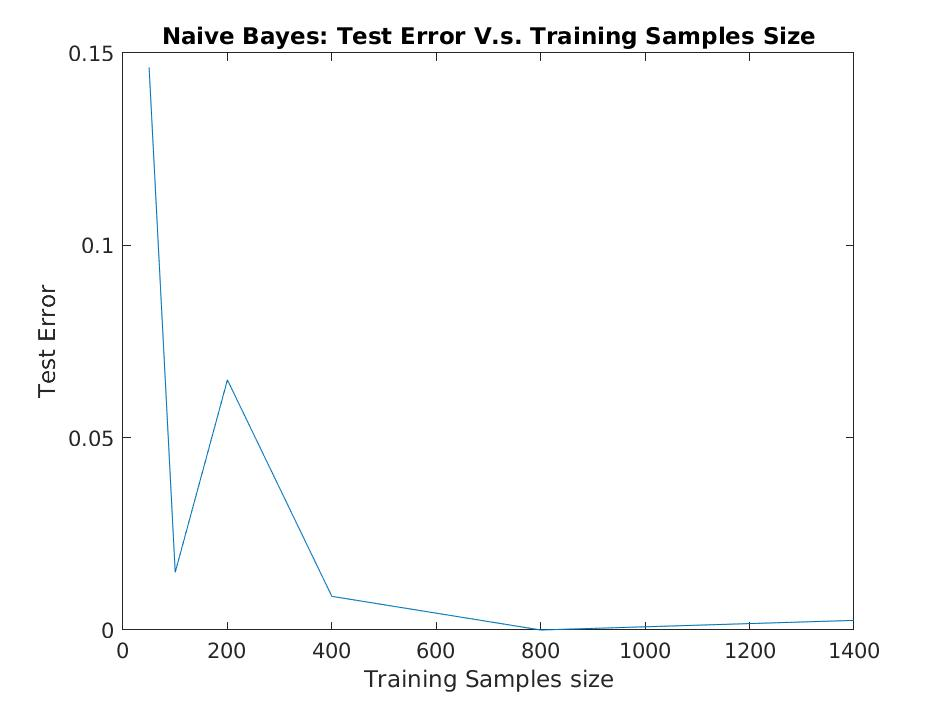
\includegraphics[width=0.5\textwidth]{cs299_ps2_p5c.jpg}
\end{center}
When the training process hits 800, the test error are smallest, zero.
}
\subsubsection{d}{
\begin{center}
      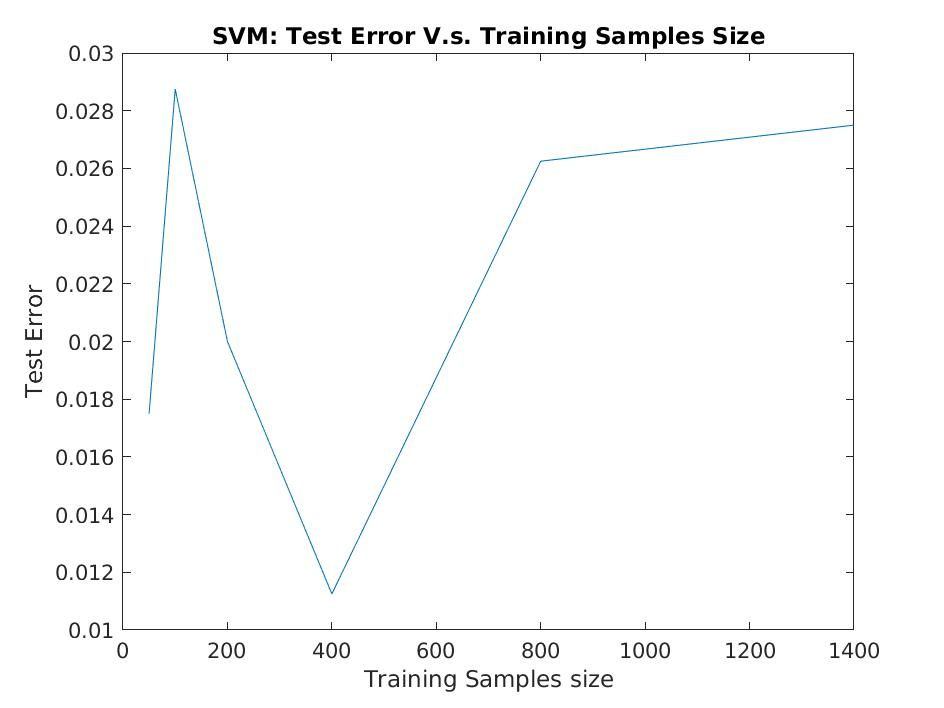
\includegraphics[width=0.5\textwidth]{cs299_ps2_p5d.jpg}
\end{center}
When the training process hits 400, the test error are smallest, zero.
}
\subsection{e}{
    Naive Bayes' training process is to count out the probability with a greater amount of sampling. So it is not easy to be over-fitted when tested. But SVM is to draw a separating planes. The chances to overfit the training dataset is very high.
}
\end{homeworkProblem}
%---------------------------------------------------------------------------------------
\end{document}
